\documentclass{article}
\usepackage{tikz}
\usetikzlibrary{arrows.meta,positioning,calc,shapes.geometric}
\pagestyle{empty}
\begin{document}
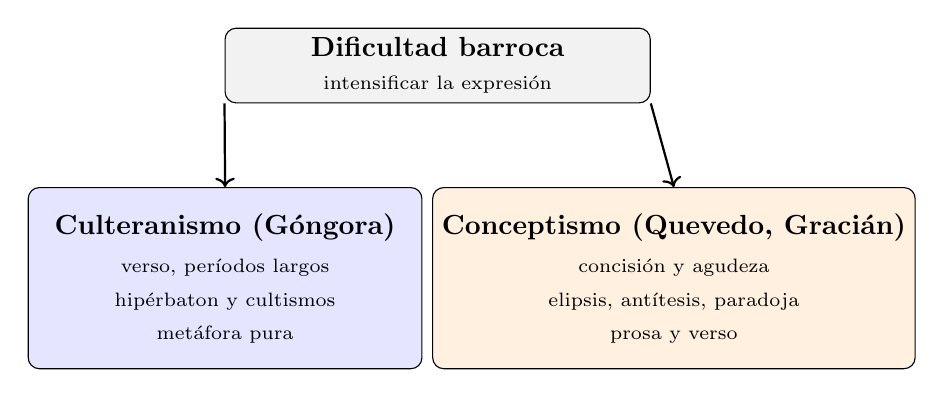
\begin{tikzpicture}
\tikzset{every node/.append style={align=center}}

\node[draw, rounded corners, fill=gray!10, minimum width=5.4cm, minimum height=0.9cm, align=center] (b) at (4.5,2.7) {\textbf{Dificultad barroca}\\ \scriptsize intensificar la expresión};
\node[draw, rounded corners, fill=blue!10, minimum width=5.0cm, minimum height=2.3cm, align=center] (c) at (1.8,0) {\textbf{Culteranismo (Góngora)}\\[2pt] \scriptsize verso, períodos largos\\ \scriptsize hipérbaton y cultismos\\ \scriptsize metáfora pura};
\node[draw, rounded corners, fill=orange!12, minimum width=5.0cm, minimum height=2.3cm, align=center] (k) at (7.5,0) {\textbf{Conceptismo (Quevedo, Gracián)}\\[2pt] \scriptsize concisión y agudeza\\ \scriptsize elipsis, antítesis, paradoja\\ \scriptsize prosa y verso};
\draw[->, thick] (b.south west) -- (c.north); \draw[->, thick] (b.south east) -- (k.north);

\end{tikzpicture}
\end{document}
